\documentclass[12pt]{article}
\usepackage[utf8]{inputenc}
\usepackage[left=2cm,right=2cm,top=2cm,bottom=2cm]{geometry}
\usepackage[spanish]{babel}
\usepackage{graphicx, amsmath, multirow}
\usepackage[small]{caption}
\usepackage{subcaption}
\usepackage{url}
\setlength{\parskip}{\baselineskip}
\graphicspath{ {images/} }

\spanishdecimal{.}
\usepackage{hyperref}
\hypersetup{
	colorlinks=true,
	linkcolor=blue,     
	urlcolor=blue,
	citecolor=blue,
}


\begin{document}

	\thispagestyle{empty}

	\begin{center}
		{\Large \bf Prueba de Chi cuadrada y covarianza}\\
		Gabriela S\'anchez Y.\\
		5064
	\end{center}
  
  	El presente trabajo se divide en secciones, cada una de ellas se enfoca en un objetivo en particular. %La sección \ref{convolucion} muestra una aplicación de la convolución, 
  	La sección \ref{pchi} presenta una aplicación de la prueba de Chi cuadrada y finalmente la sección \ref{covarianza} valida de forma numérica y analítica dos propiedades relacionadas a la covarianza.
  	
  	Los experimentos realizados para encontrar los resultados numéricos se realizan con el apoyo del lenguaje de programación \textsc{R} \cite{rstatistics} cuyo código puede consultarse en el archivo \texttt{t11.R} \cite{mpa_gaby}.
  	
  	%se simulan problemas previamente que previamente se resolvieron de forma analítica \cite{mpa_gabyt9}, con el objetivo de encontrar evidencia numérica que apoye el resultado analítico. Las simulaciones se realizan con el apoyo del lenguaje de programación \textsc{R} \cite{rstatistics}. .
	
	%\section{Convolución} \label{convolucion}
	
	\section{Prueba de Chi cuadrada} \label{pchi}
	
	Existen varios tipos de pruebas de Chi cuadrada: la prueba de bondad de ajuste y las pruebas de asociación e independencia. La prueba de bondad de ajuste se utiliza para probar qué tan bien se ajusta una muestra de datos categóricos a una distribución teórica. Las pruebas de asociación e independencia, tal y como su nombre lo dice, se usan para determinar si una variable está asociada con otra y para determinar si el valor observado de una variable depende del valor observado de otra, respectivamente \cite{minitab}.
	
	Por el momento no fue posible determinar una aplicación de esta prueba a los datos actuales de la tesis por lo que se usan los datos proporcionados por el INEGI \cite{inegi} sobre Seguridad pública y justicia. Específicamente datos sobre la percepción de la población mayor de 18 años, por tipo de autoridad. Se tienen dos tipos de percepción {\em algo efectivo} y {\em muy efectivo} y se analizan sólo dos tipos de autoridad: policía federal y estatal. Los datos se muestran en el cuadro \ref{dtaos-chi}.
	
	\begin{table}[h]
		\centering
		\caption{Percepción de la efectividad del trabajo de diferentes tipos de autoridades.}
		\label{dtaos-chi}
		\begin{tabular}{lrr}
			\hline
			& Muy efectivo & Algo efectivo\\
			\hline
			Policía federal & 16.3 & 49.7 \\
			Policía estatal & 8.7 & 45.1 \\
			\hline
		\end{tabular}
	\end{table}
	
	Con estos datos, se aplica la prueba de asociación de Chi cuadrada para determinar si el tipo de autoridad afecta al nivel de percepción. La hipótesis nula es que no hay asociación entre estas dos variables, es decir, que el tipo de autoridad no se asocia con la percepción de efectividad. Para poder analizar el valor de {\em chi cuadrada}, primero se aclara que se tiene una tabla de valores de $2 \times 2$, es decir, se tienen dos grados de libertad. En este caso el valor crítico con el que se compara el valor de {\em chi cuadrada} es 3.841. 
	
	Los resultados obtenidos se muestran a continuación:
	\begin{verbatim}
	Pearson's Chi-squared test
	
	data:  prueba
	X-squared = 1.3047, df = 1, p-value = 0.2534
	\end{verbatim}
	
	El $p$-valor es mayor que el nivel de significación, lo que indica que no se puede rechazar la hipótesis nula. Observe también que {\em chi cuadrada} $<$ 3.841, de acuerdo a esto, la hipótesis nula no se rechaza.
	
	\section{Covarianza} \label{covarianza}
	
	En esta sección se desea validar de forma numérica y analítica dos propiedades relacionadas a la covarianza. Para lograr el objetivo, primero es necesario definir la covarianza, recordar el concepto de varianza y algunas propiedades del valor esperado. En adelante $\mu_x$ y $\mu_y$ representan el valor esperado de las variables aleatorias $X$ y $Y,$ respectivamente
	
	Sean $X$ y $Y$ dos variables aleatorias, la covarianza de éstas se define mediante la ecuación \ref{cov1} o, de manera alternativa, mediante la ecuación \ref{cov2}
	\begin{eqnarray}
	\text{Cov}[X,Y] &=& E[(X-\mu_x)(Y-\mu_y)] 	\label{cov1} \\
	&=& E[XY] - \mu_x\mu_y. \label{cov2}
	\end{eqnarray}	
	
	Por su parte, la varianza de una variable aleatoria $X$ se define por la ecuación \ref{var}
	\begin{equation}
	V[X] = E[(X - \mu_x)^2] = E[X^2] - \mu_x^2.
	\label{var}
	\end{equation}
	
	El valor esperado cumple con diferentes propiedades \cite{prob2003}: el valor esperado de la suma de dos variables aleatorias es la suma de los valores esperados y el valor esperado de una variable aleatoria multiplicada por una constante es esa constante multiplicada por el valor valor esperado de la variable aleatoria. Es decir,
	\begin{eqnarray}
	E[X + Y] &=& E[X] + E[Y], \label{esuma}\\
	E[cX] &=& cE[X] \label{econst}.
	\end{eqnarray} 
	
	\subsection{Propiedad 1}
	
	Primero se demuestra que $\text{Cov}[aX+b, cY+d] = ac \cdot \text{Cov}[X,Y]$ de forma analítica. De acuerdo a la definición de covarianza, es necesario calcular el valor esperado de las variables $aX+b$ y $cY+d$. De esta manera, utilizando las propiedades del valor esperado, se tiene que
	\begin{equation*}
	E[aX+b] = E[aX]+ E[b] = aE[X] + b = a\mu_x + b,
	\end{equation*}
	procediendo de manera análoga se puede determinar que $E[cY+d] = c\mu_y + d$. Entonces
	\begin{eqnarray*}
		\text{Cov}[aX+b, cY+d] &=& E[\{aX+b - (a\mu_x + b)\}\{cY+d - (c\mu_y + d)\}] \\
		&=& E[(aX - a\mu_x) (cY - c\mu_y)] \\	
		&=& E[acXY - ac\mu_xY - ac\mu_yX + ac\mu_x\mu_y] \\
		&=& ac \cdot E[XY - \mu_xY - \mu_yX + \mu_x\mu_y] \\
		&=& ac \cdot E[(X - \mu_x)(Y - \mu_y)] \\
		&=& ac \cdot Cov[X,Y].
	\end{eqnarray*}

	La demostración numérica consiste en tomar, para la variable $X$ mil elementos que siguen una distribución de probabilidad normal con media cero y desviación estándar igual a cinco. Mientras que los elementos de la variable $Y$ siguen una distribución uniforme. Después se crean las variables aleatorias $aX+b$ y $cY+d$. 
	
	Sin perder la generalidad se definen $a=3$, $b=1$, $c=5$ y $d=2$. Se calculan por separado $\text{Cov}[aX+b, cY+d]$ y $ac \cdot Cov[X,Y]$ mediante el uso de la función \texttt{cov} de \textsc{R}. El procedimiento se repite cien veces y los resultados se muestran en los histogramas de la figura \ref{cov}. Prácticamente se tiene el mismo histograma por lo que se puede concluir que la propiedad sí se cumple.
	
	\begin{figure}
		\begin{subfigure}{0.5\textwidth}
			\centering
			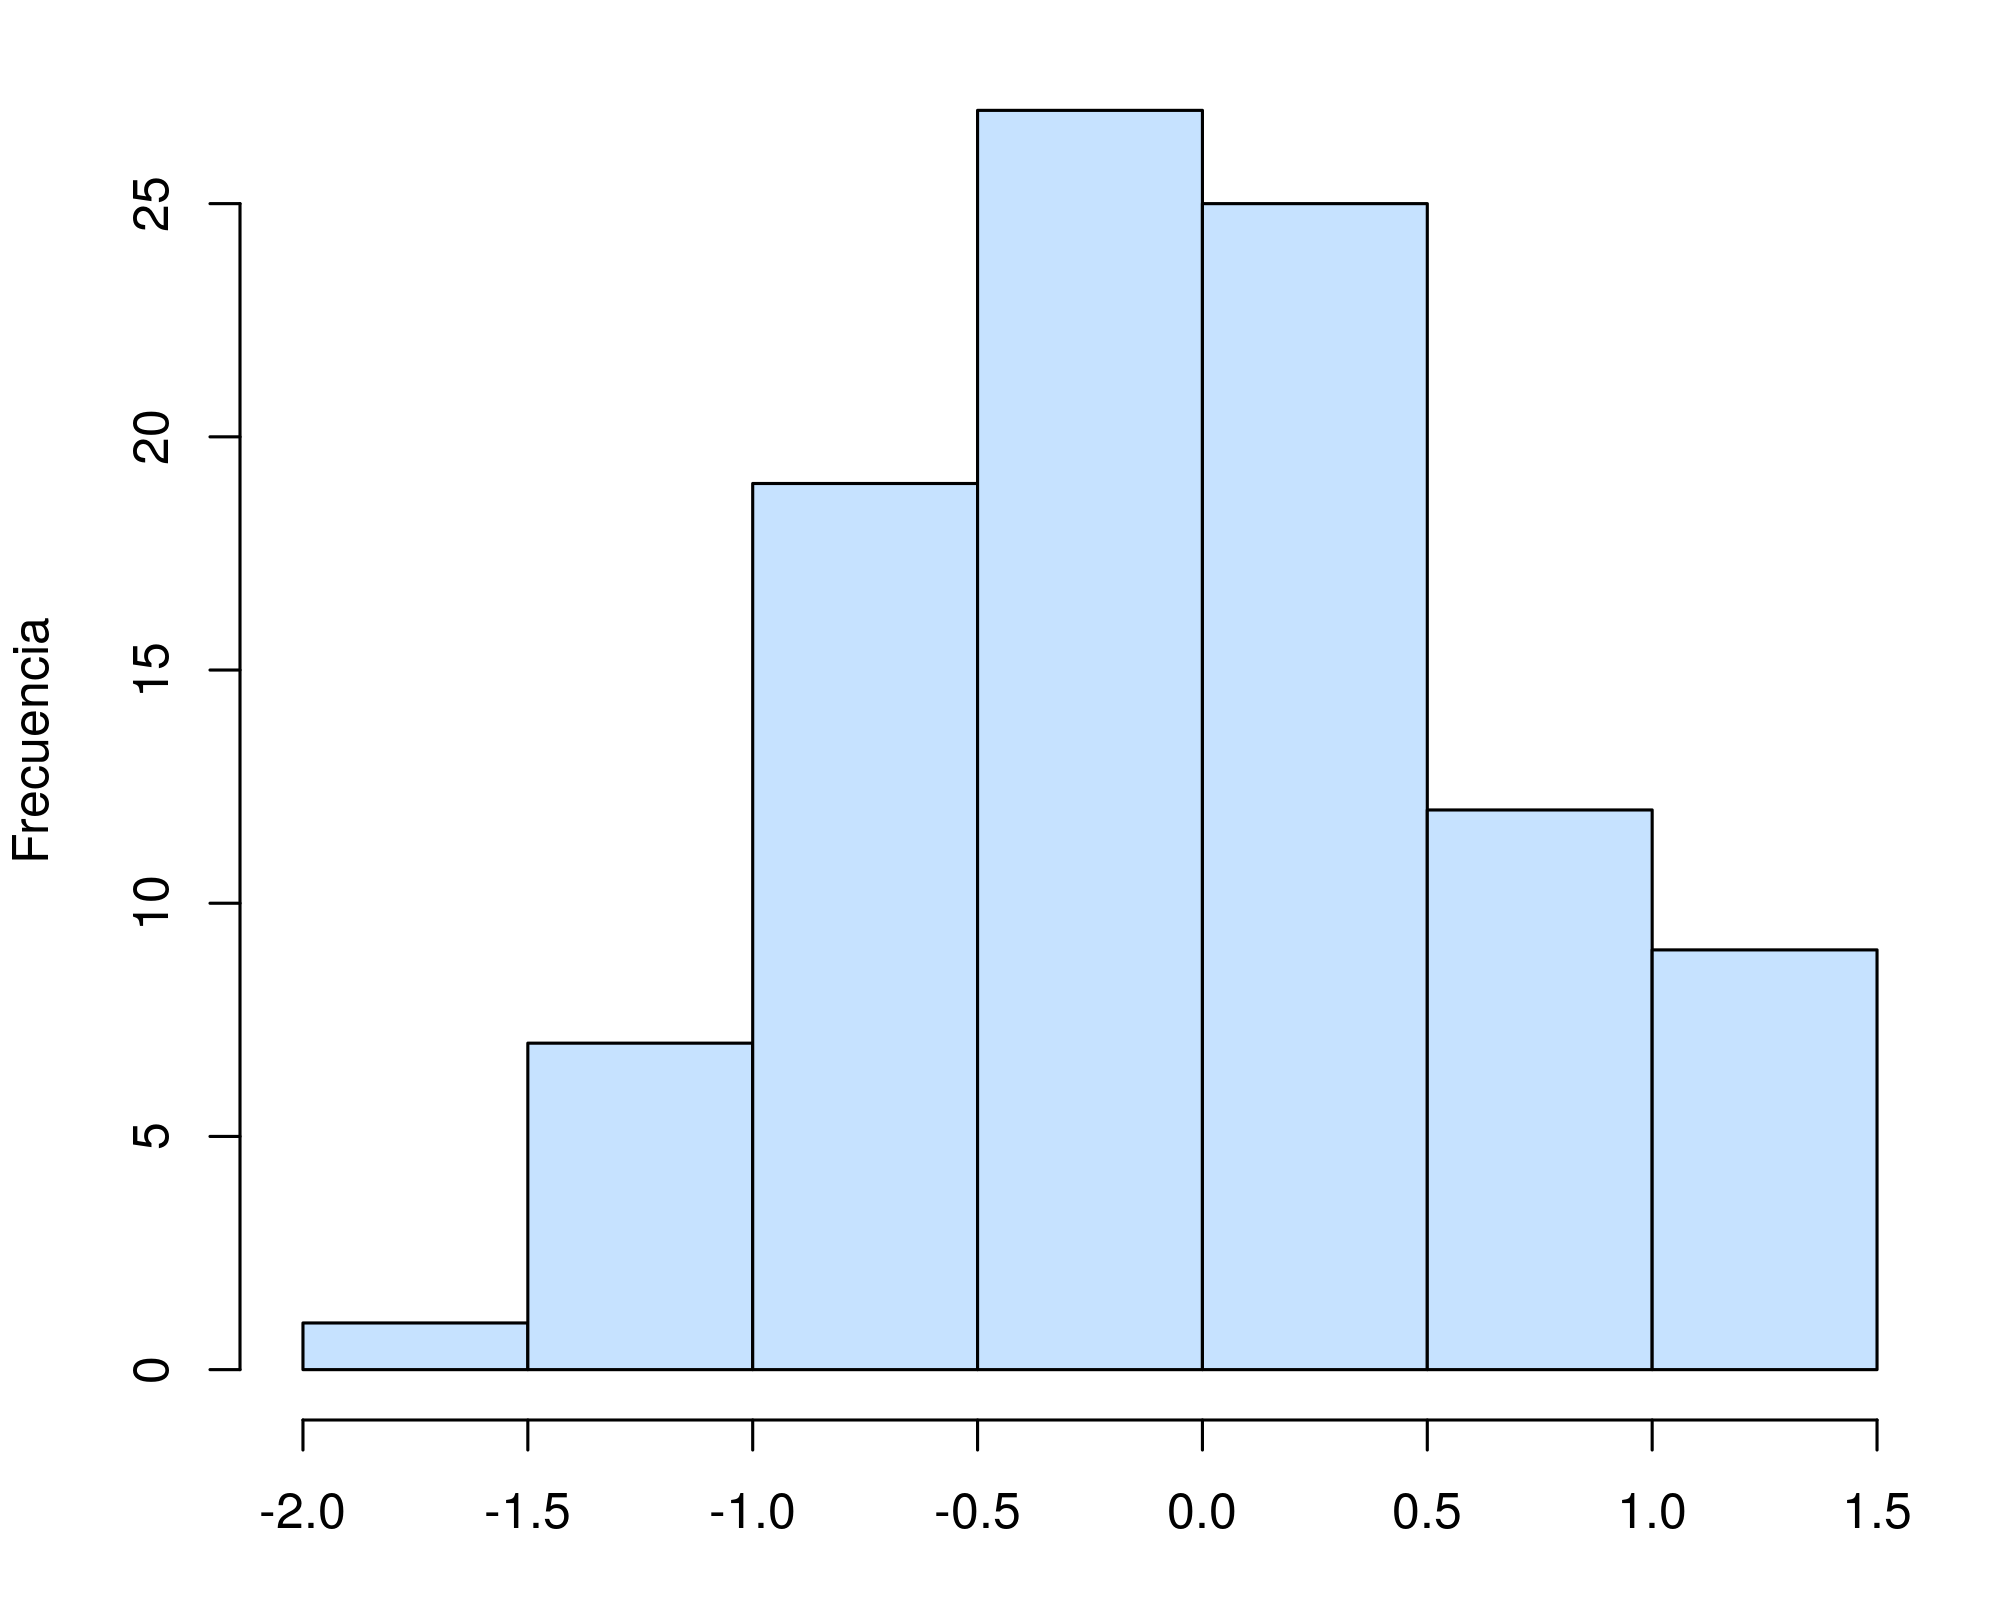
\includegraphics[scale=0.5]{cov_abcd.png}
			\caption{$\text{Cov}[aX+b, cY+d]$}
		\end{subfigure}
		\begin{subfigure}{0.5\textwidth}
			\centering
			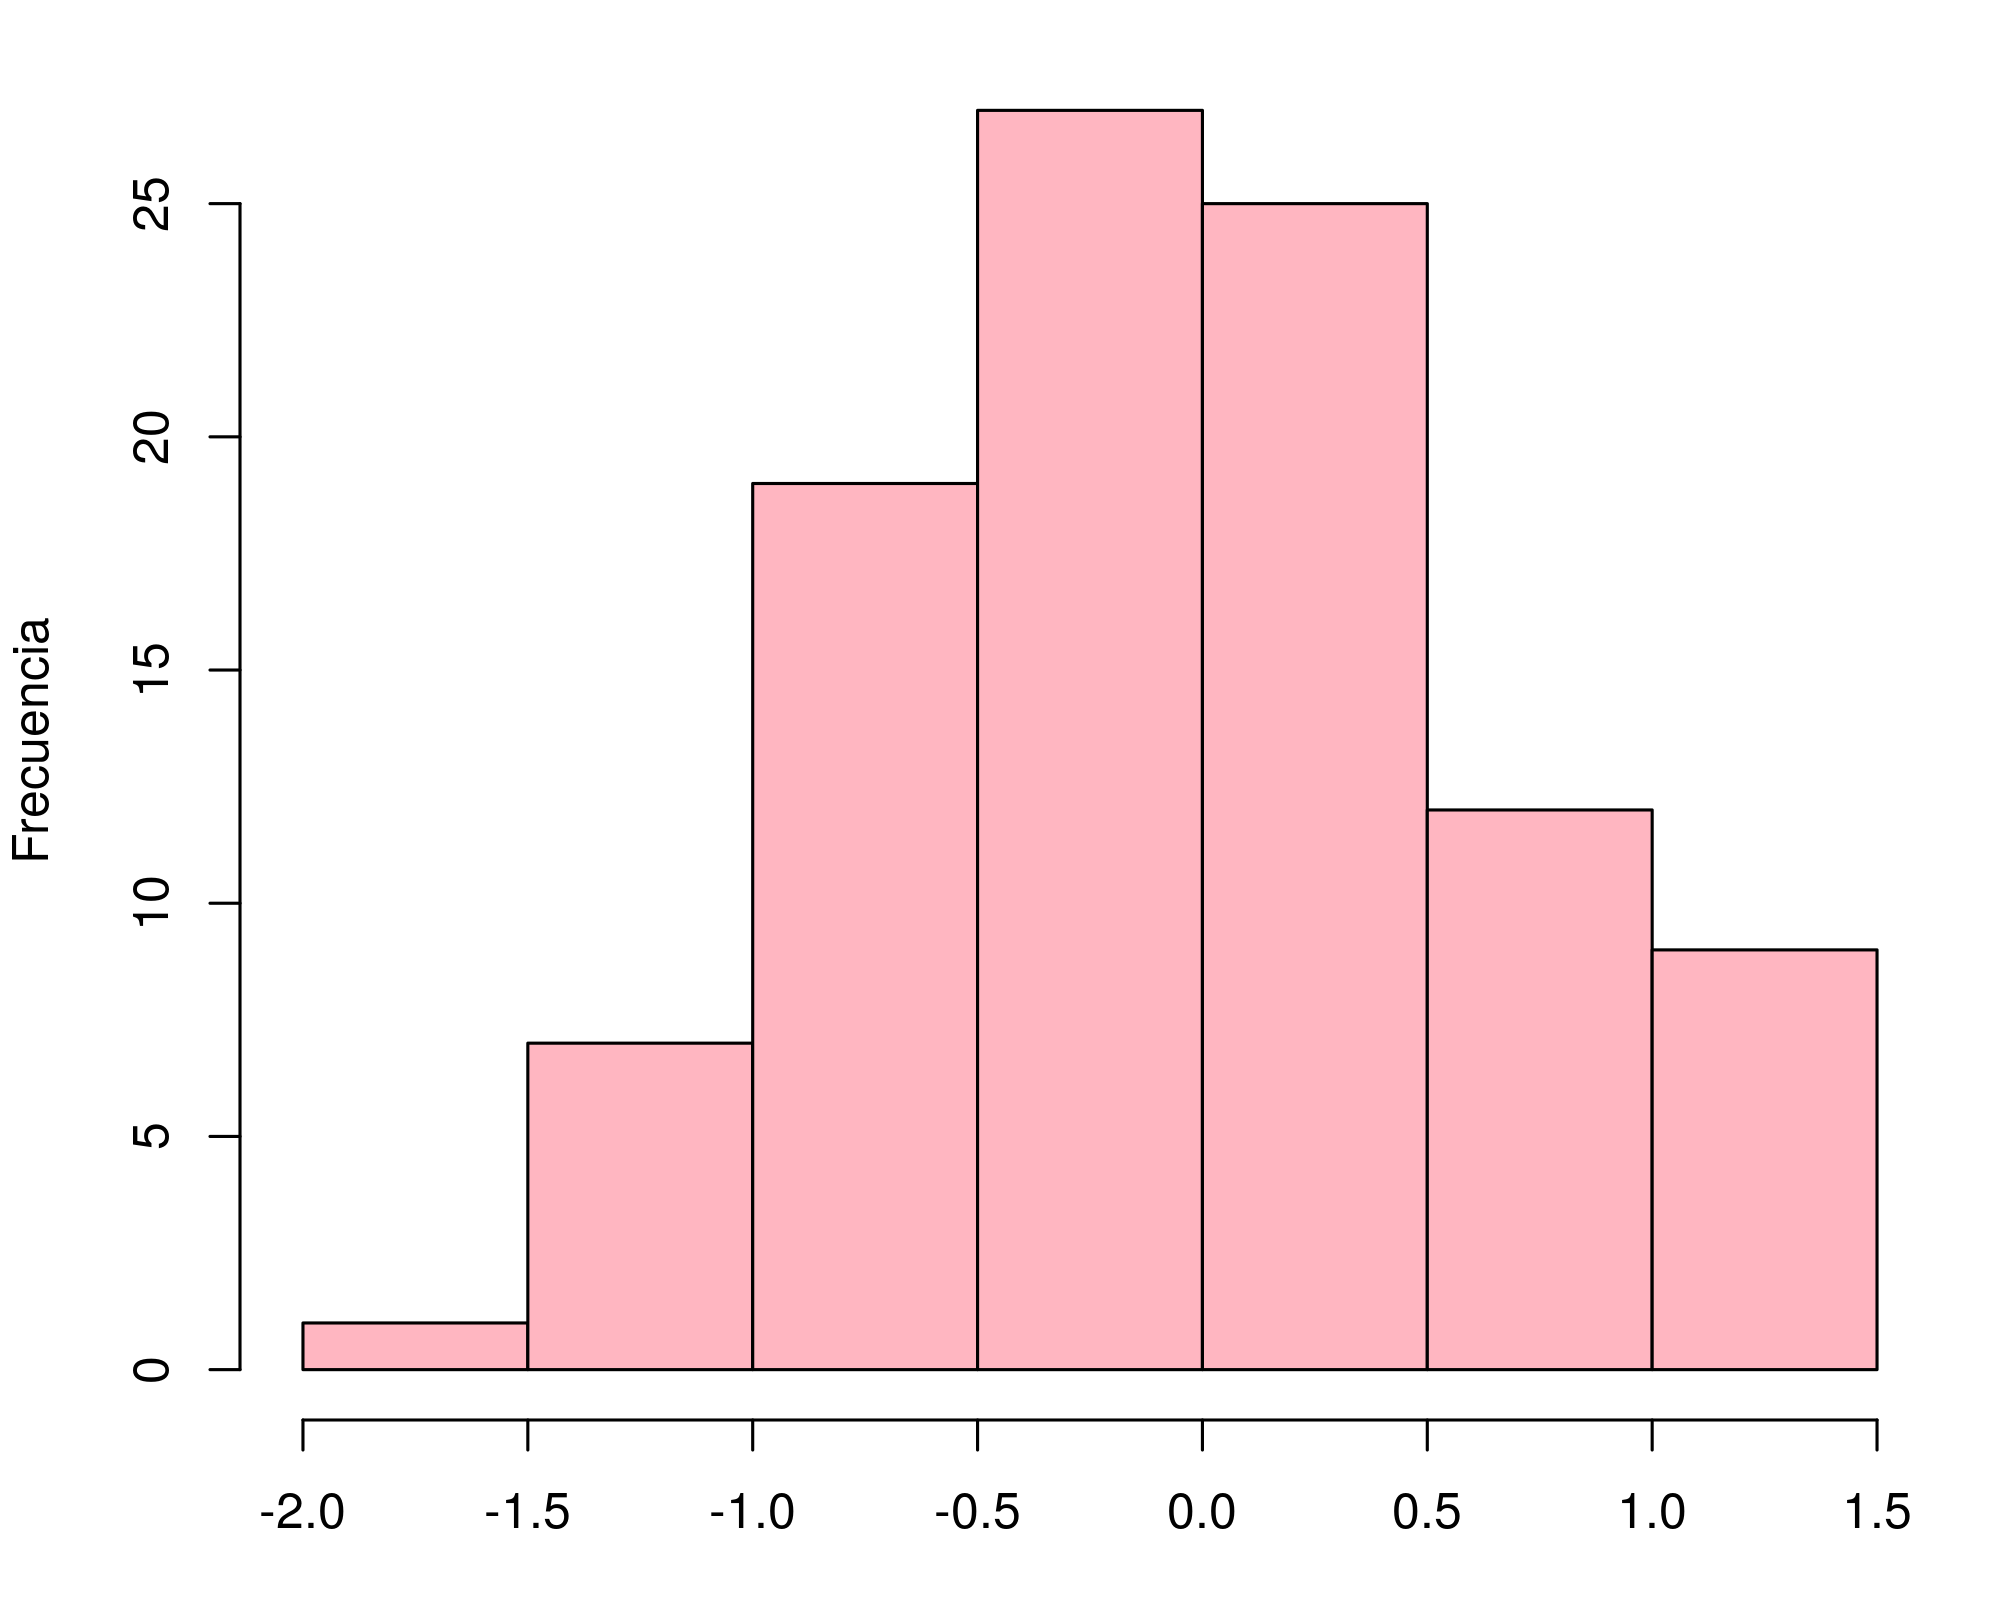
\includegraphics[scale=0.5]{cov_ac.png}
			\caption{$ac \cdot Cov[X,Y]$}
		\end{subfigure}
		\caption{Demostración numérica de la propiedad  $\text{Cov}[aX+b, cY+d] = ac \cdot \text{Cov}[X,Y]$.}
		\label{var}
	\end{figure}

	\subsection{Propiedad 2}

	Se desea demostrar que $\text{Var}[X+Y] = \text{Var}[X] + \text{Var}[Y] + 2\text{Cov}[X, Y]$. Dada la definición de varianza, es necesario encontrar el valor esperado de la suma de las variables aleatorias $X$ y $Y$:
	\begin{equation*}
	E[X+Y] = E[X] + E[Y] = \mu_x + \mu_y.
	\end{equation*}
	Con este resultado, se procede a la demostración de la propiedad
	\begin{eqnarray*}
	\text{Var}[X+Y] &=& E[(X + Y - \mu_x - \mu_y)^2] \\
	&=& E[X^2 + XY - \mu_xX - \mu_yX + YX + Y^2 - \mu_xY - \mu_yY - \mu_xX - \mu_xY + \mu_x^2 + \\
	& & \mu_x\mu_y - \mu_yX - \mu_yY + \mu_x\mu_y + \mu_y^2] \\
	&=& E[X^2 + 2XY - 2\mu_xX - 2\mu_yX - 2\mu_xY - 2\mu_yY + 2\mu_x\mu_y + \mu_x^2 + \mu_y^2 + Y^2] \\
	&=& E[X^2 - 2\mu_xX + \mu_x^2] + E[Y^2 - 2\mu_yY + \mu_y^2] + E[2XY - 2\mu_yX - 2\mu_xY + 2\mu_x\mu_y] \\
	&=& E[(X - \mu_x)^2] + E[(Y-\mu_y)^2] + 2E[(X-\mu_x)(Y-\mu_y)] \\
	&=& \text{Var}[X] + \text{Var}[Y] + 2\text{Cov}[X, Y].
	\end{eqnarray*}

	La demostración numérica sigue una idea similar a la planteada para demostrar la propiedad 1. Nuevamente se definen $X\sim Norm(0,5)$ y $Y \sim Norm(0,1)$. Mediante las funciones \texttt{var} y \texttt{cov} de \textsc{R} se realiza el cálculo de $\text{Var}[X+Y]$ y $\text{Var}[X] + \text{Var}[Y] + 2\text{Cov}[X, Y]$. El proceso se repite un total de cien veces cuyos resultados se presentan en los histogramas de la figura \ref{var}. En este experimento, nuevamente se observa que se obtienen los mismos resultados en cada cálculo de manera que se apoya la demostración de la propiedad 2.
	
	\begin{figure}
		\begin{subfigure}{0.5\textwidth}
			\centering
			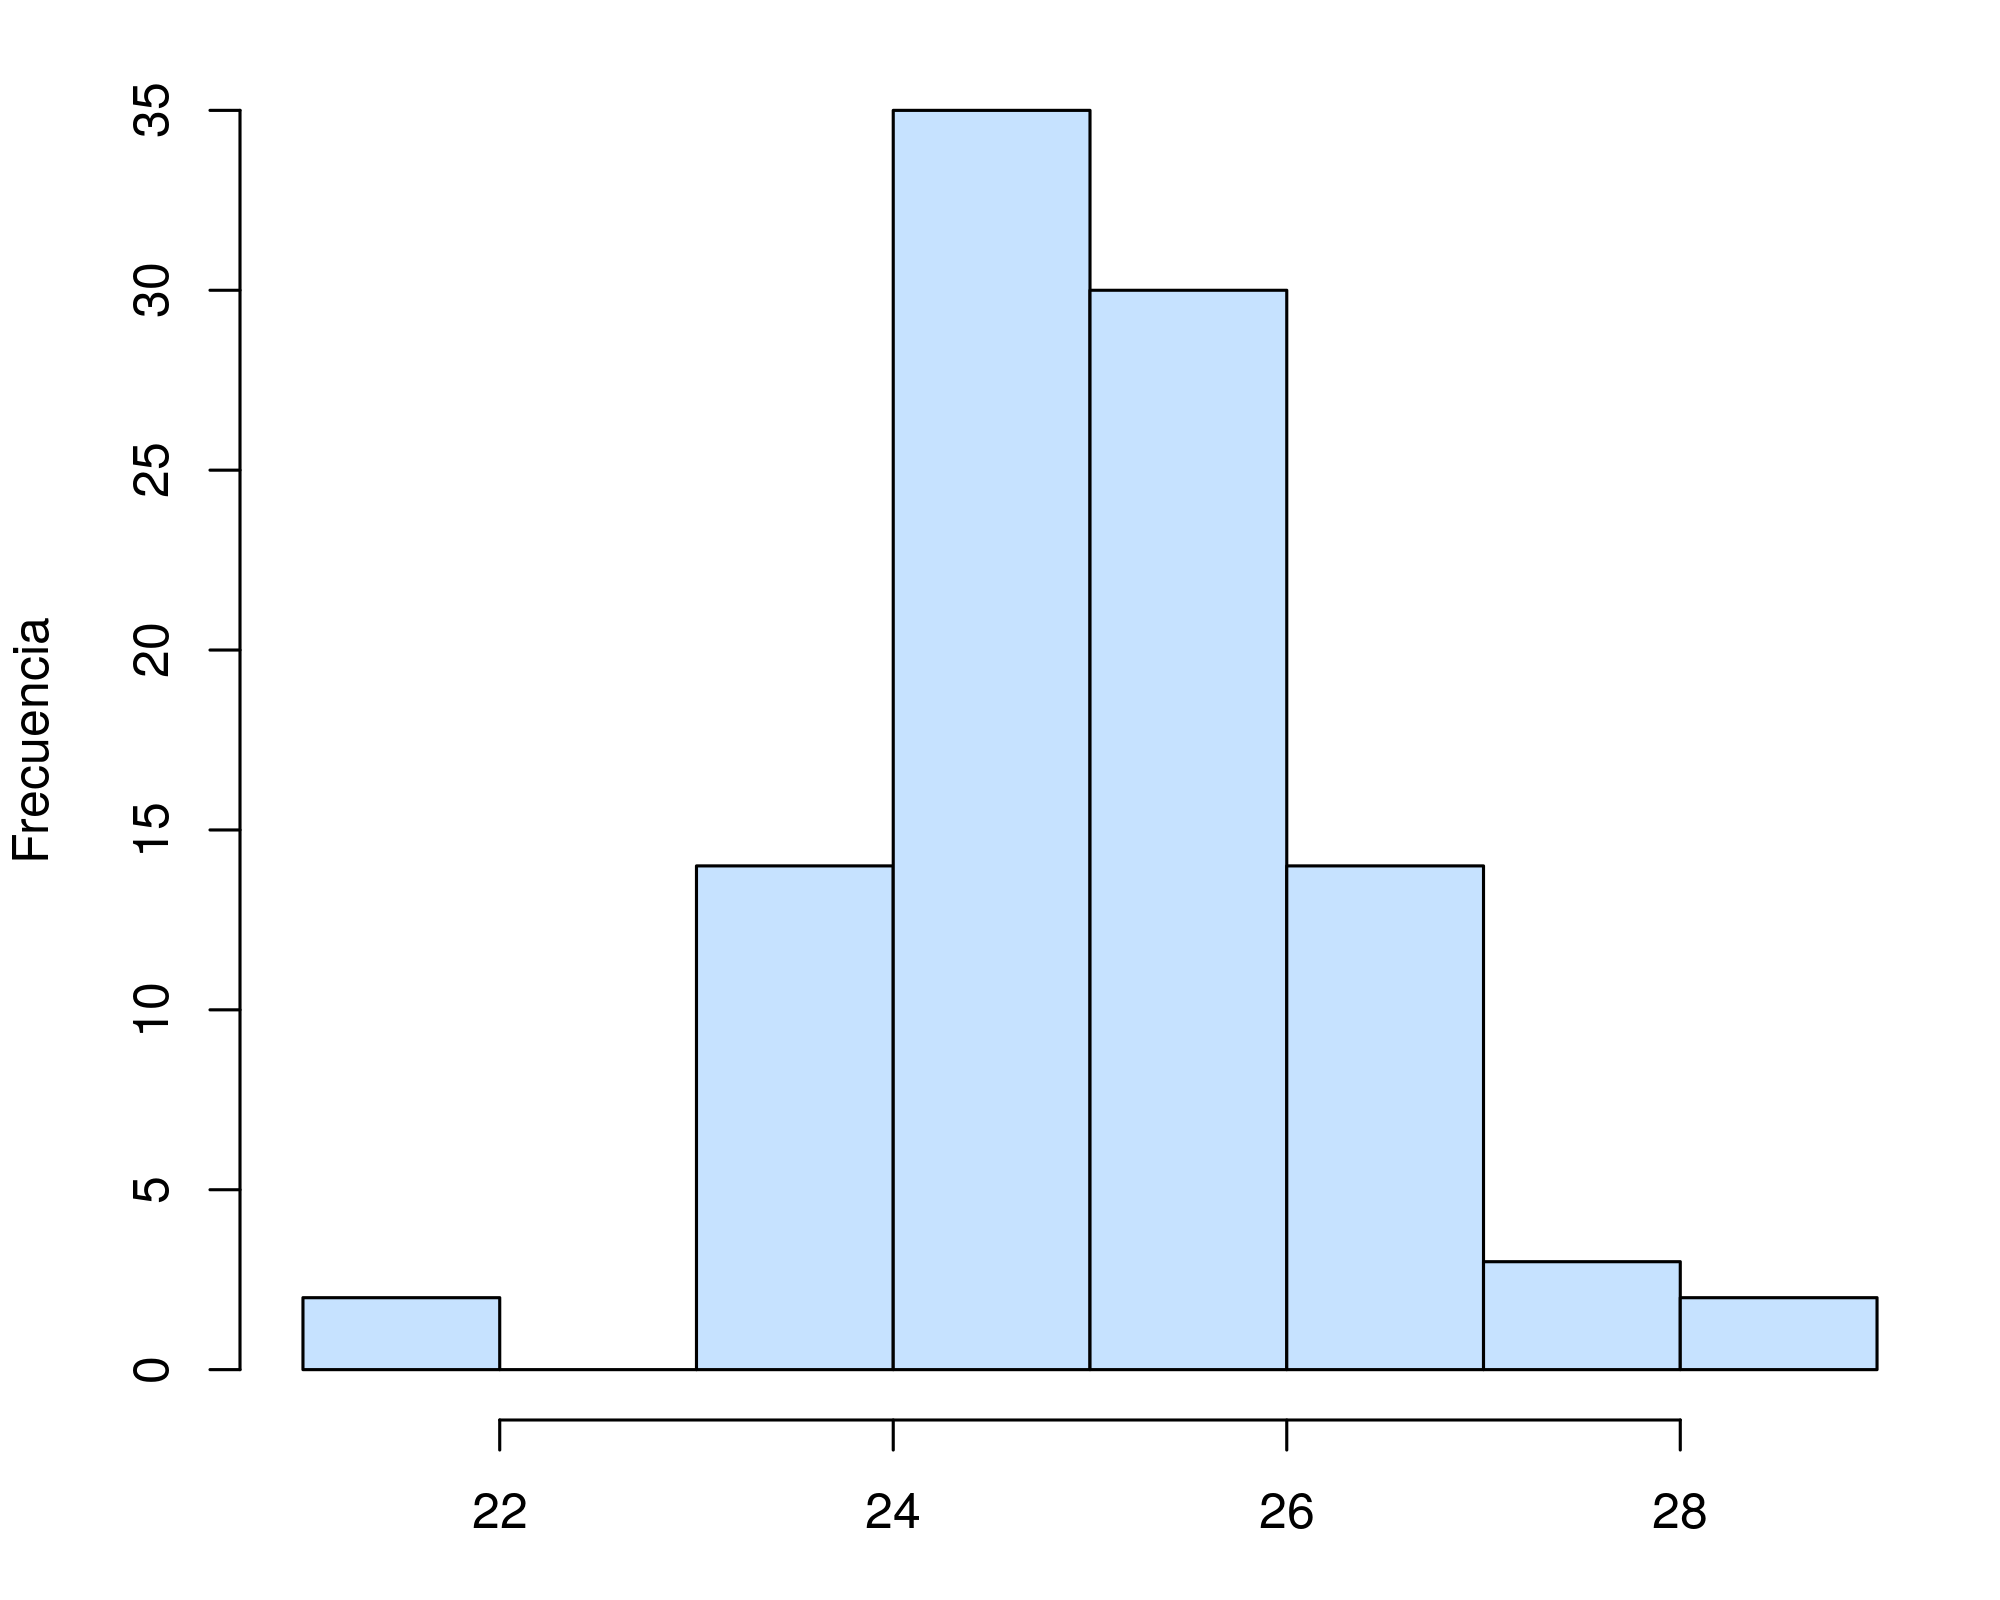
\includegraphics[scale=0.5]{var_suma.png}
			\caption{$\text{Var}[X+Y]$}
		\end{subfigure}
		\begin{subfigure}{0.5\textwidth}
			\centering
			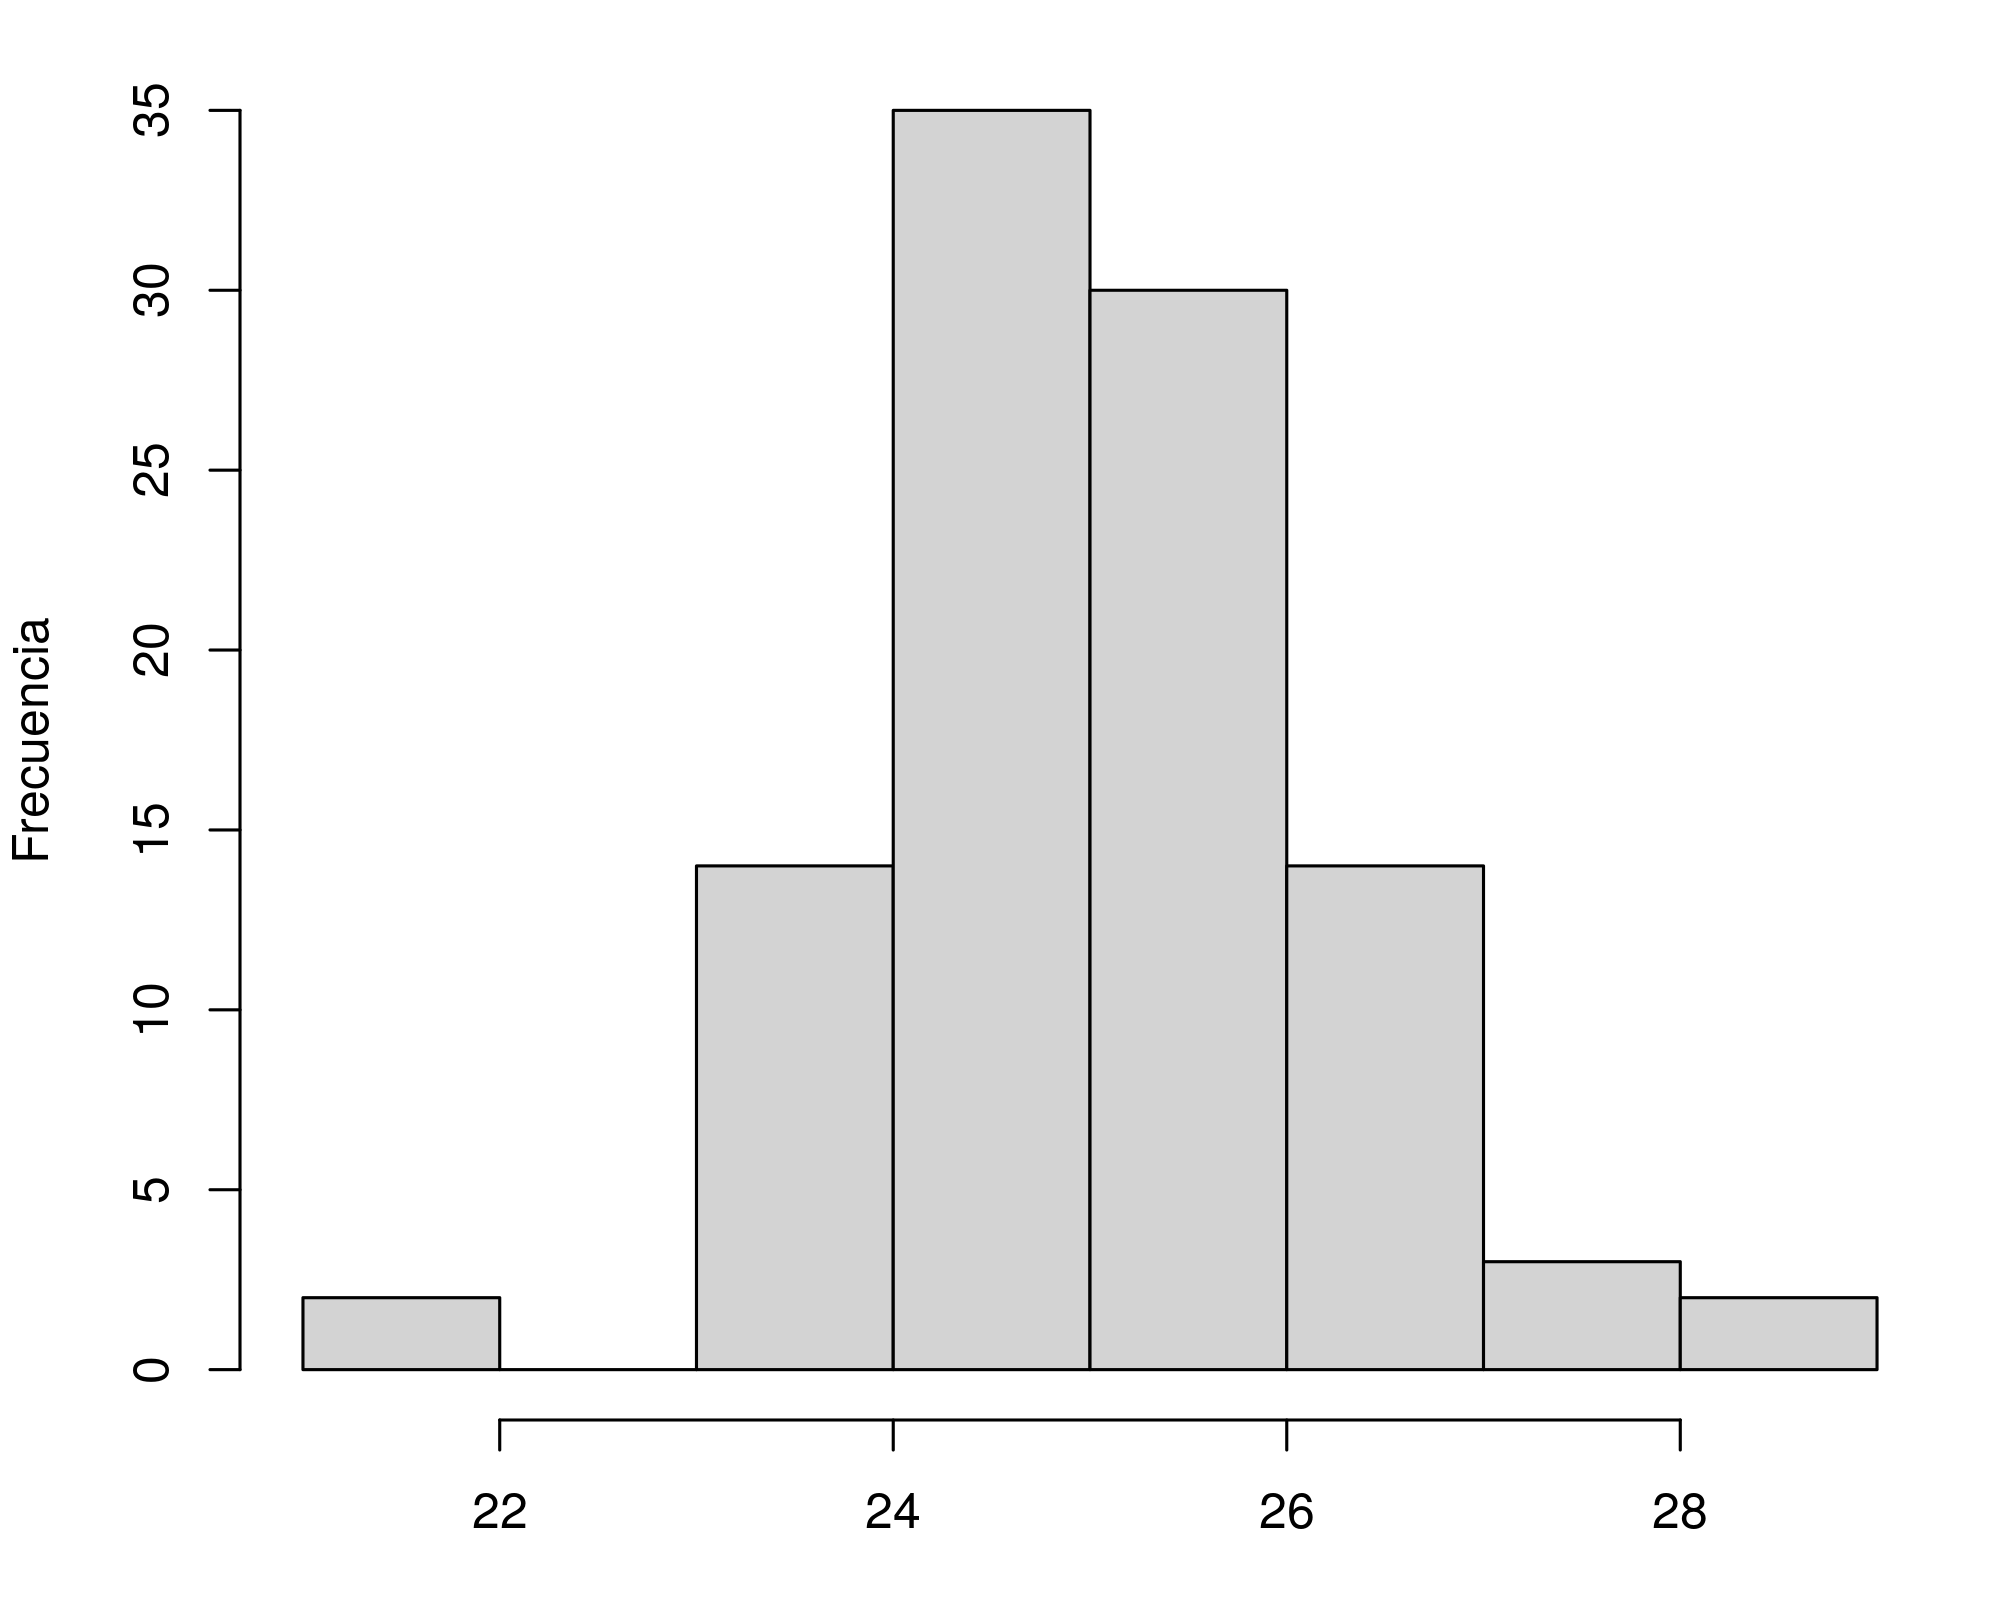
\includegraphics[scale=0.5]{var_resultado.png}
			\caption{$\text{Var}[X] + \text{Var}[Y] + 2\text{Cov}[X, Y]$}
		\end{subfigure}
		\caption{Demostración numérica de la propiedad  $\text{Var}[X+Y] = \text{Var}[X] + \text{Var}[Y] + 2\text{Cov}[X, Y]$.}
		\label{cov}
	\end{figure}
	
\bibliographystyle{plain}
\bibliography{biblio}

\end{document}
